\documentclass{article}

\usepackage{amsmath, amsthm, amssymb, amsfonts}
\usepackage{thmtools}
\usepackage{graphicx}
\usepackage{setspace}
\usepackage{geometry}
\usepackage{float}
\usepackage{hyperref}
\usepackage[utf8]{inputenc}
\usepackage[english]{babel}
\usepackage{framed}
\usepackage[dvipsnames]{xcolor}
\usepackage{tcolorbox}
\usepackage{fancyhdr}
\usepackage{geometry}
\usepackage{float}
\usepackage{tabularx}
\usepackage{array}
\usepackage[table]{xcolor}
\geometry{
 a4paper,
 total={170mm,257mm},
 left=30mm,
 right=30mm,
 top=30mm,
}
\colorlet{LightGray}{White!90!Periwinkle}
\colorlet{LightOrange}{Orange!15}
\colorlet{LightGreen}{Green!15}
\pagestyle{fancy}
\fancyhf{} % Pulisce l'header e il footer predefiniti
\renewcommand{\headrulewidth}{0pt} % Opzionale: rimuove la linea orizzontale dall'header
\fancyhead[C]{\textbf{MLPR Project:\\ Fingerprint spoofing detection}} % Titolo centrato nell'header
\fancyfoot[C]{\thepage}
\newcommand{\HRule}[1]{\rule{\linewidth}{#1}}

\declaretheoremstyle[name=Theorem,]{thmsty}
\declaretheorem[style=thmsty,numberwithin=section]{theorem}
\tcolorboxenvironment{theorem}{colback=LightGray}


\declaretheoremstyle[name=Proposition,]{prosty}
\declaretheorem[style=prosty,numberlike=theorem]{proposition}
\tcolorboxenvironment{proposition}{colback=LightOrange}

\declaretheoremstyle[name=Principle,]{prcpsty}
\declaretheorem[style=prcpsty,numberlike=theorem]{principle}
\tcolorboxenvironment{principle}{colback=LightGreen}

\setstretch{1.2}
\geometry{
    textheight=9in,
    textwidth=5.5in,
    top=1in,
    headheight=12pt,
    headsep=25pt,
    footskip=30pt
}

% ------------------------------------------------------------------------------

\begin{document}

% ------------------------------------------------------------------------------
% Cover Page and ToC
% ------------------------------------------------------------------------------

\title{ \normalsize \textsc{}
		\\ [2.0cm]
		\HRule{1.5pt} \\
		\LARGE \textbf{\uppercase{Report Machine Learning and pattern recognition}
		\HRule{2.0pt} \\ [0.6cm] \LARGE{Fingerprint spoofing detection} \vspace*{10\baselineskip}}
		}
\date{}
\author{\textbf{Alessia Intini} \\ 
		s309895 \\
		Politecnico di Torino \\
		2023/24}

\maketitle
\newpage

\tableofcontents
\newpage

% ------------------------------------------------------------------------------
\noindent\textbf{The goal of project is to perform a binary classification on fingerprint spoofing detection, that is to identify genuine vs counterfeit fingerprint images. The dataset consists of labeled samples corresponding to the genuine (True, label 1) class and the fake (False, label 0) class, the data is 6-dimensional.}
\section{Dataset Analysis}
\subsection{Training and evaluation sets}
The datasets provided contain 6000 samples; the first 6 values in each row represent the features, while the last value is the label. Specifically they are: 
\begin{itemize}
    \item Training Set: 2990 samples beloging to the Fake class (label 0) and 3010 samples belonging to the Genuine class (label 1)
    \item Evaluation Set: 3010 samples beloging to the Fake class (label 0) and 2990 samples belonging to the Genuine class (label 1)
\end{itemize}
We will use the Training Set to perform all the analysis, during this phase the dataset is divided to use about 60\% of it as the training dataset and the remaining 40\% for validation. 
After this step, the most promising models were chosen and the evaluation dataset was used to evaluate them and make the final considerations.
\subsection{Features analysis}
We can start to analize all features, here is the graph of each feature, through these histograms it is shown how each feature is distributed:\\
\begin{figure}[ht]
        \centering
        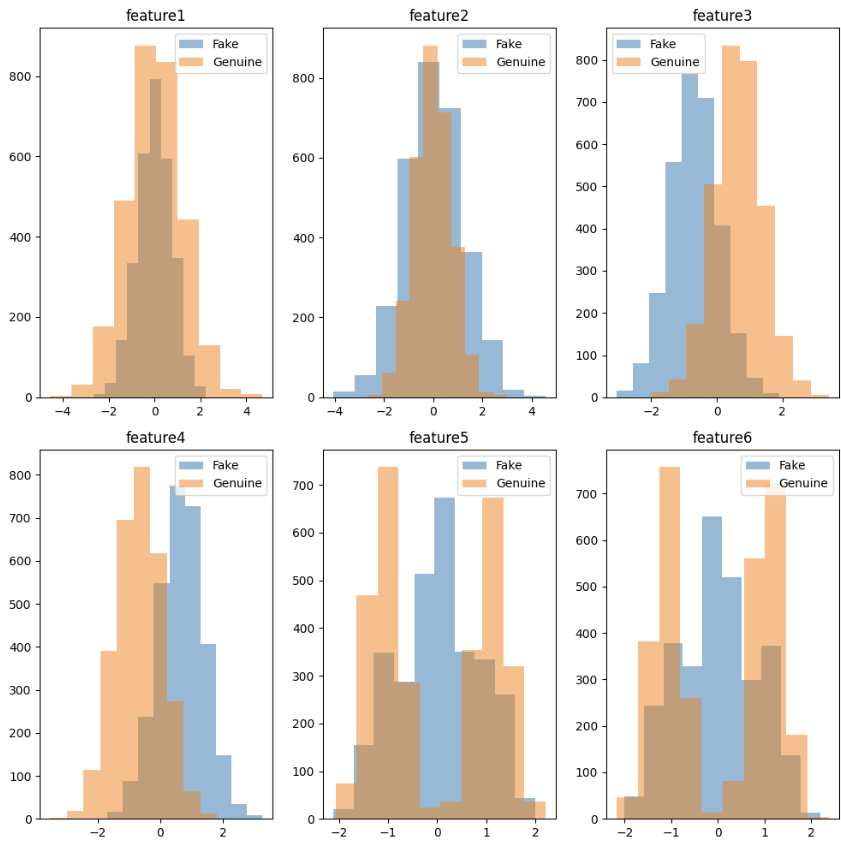
\includegraphics[width=0.5\textwidth]{./img/AllFeatures.png}
        \caption{All features}
        \label{fig:AllFeatures}
\end{figure}  
\\
By plotting a histogram for each feature, separately for the Fake and Genuine classes, it is possible to show whether the samples follow a Gaussian distribution and to what extent. 
Thus, we can say that some features follow a Gaussian distribution. Furthermore, it can be seen that features 4 and 5 may be the most discriminating features based on their ability to separate the data of the two classes.\\
\begin{figure}[ht]
    \begin{minipage}[b]{0.45\textwidth}
        \centering
        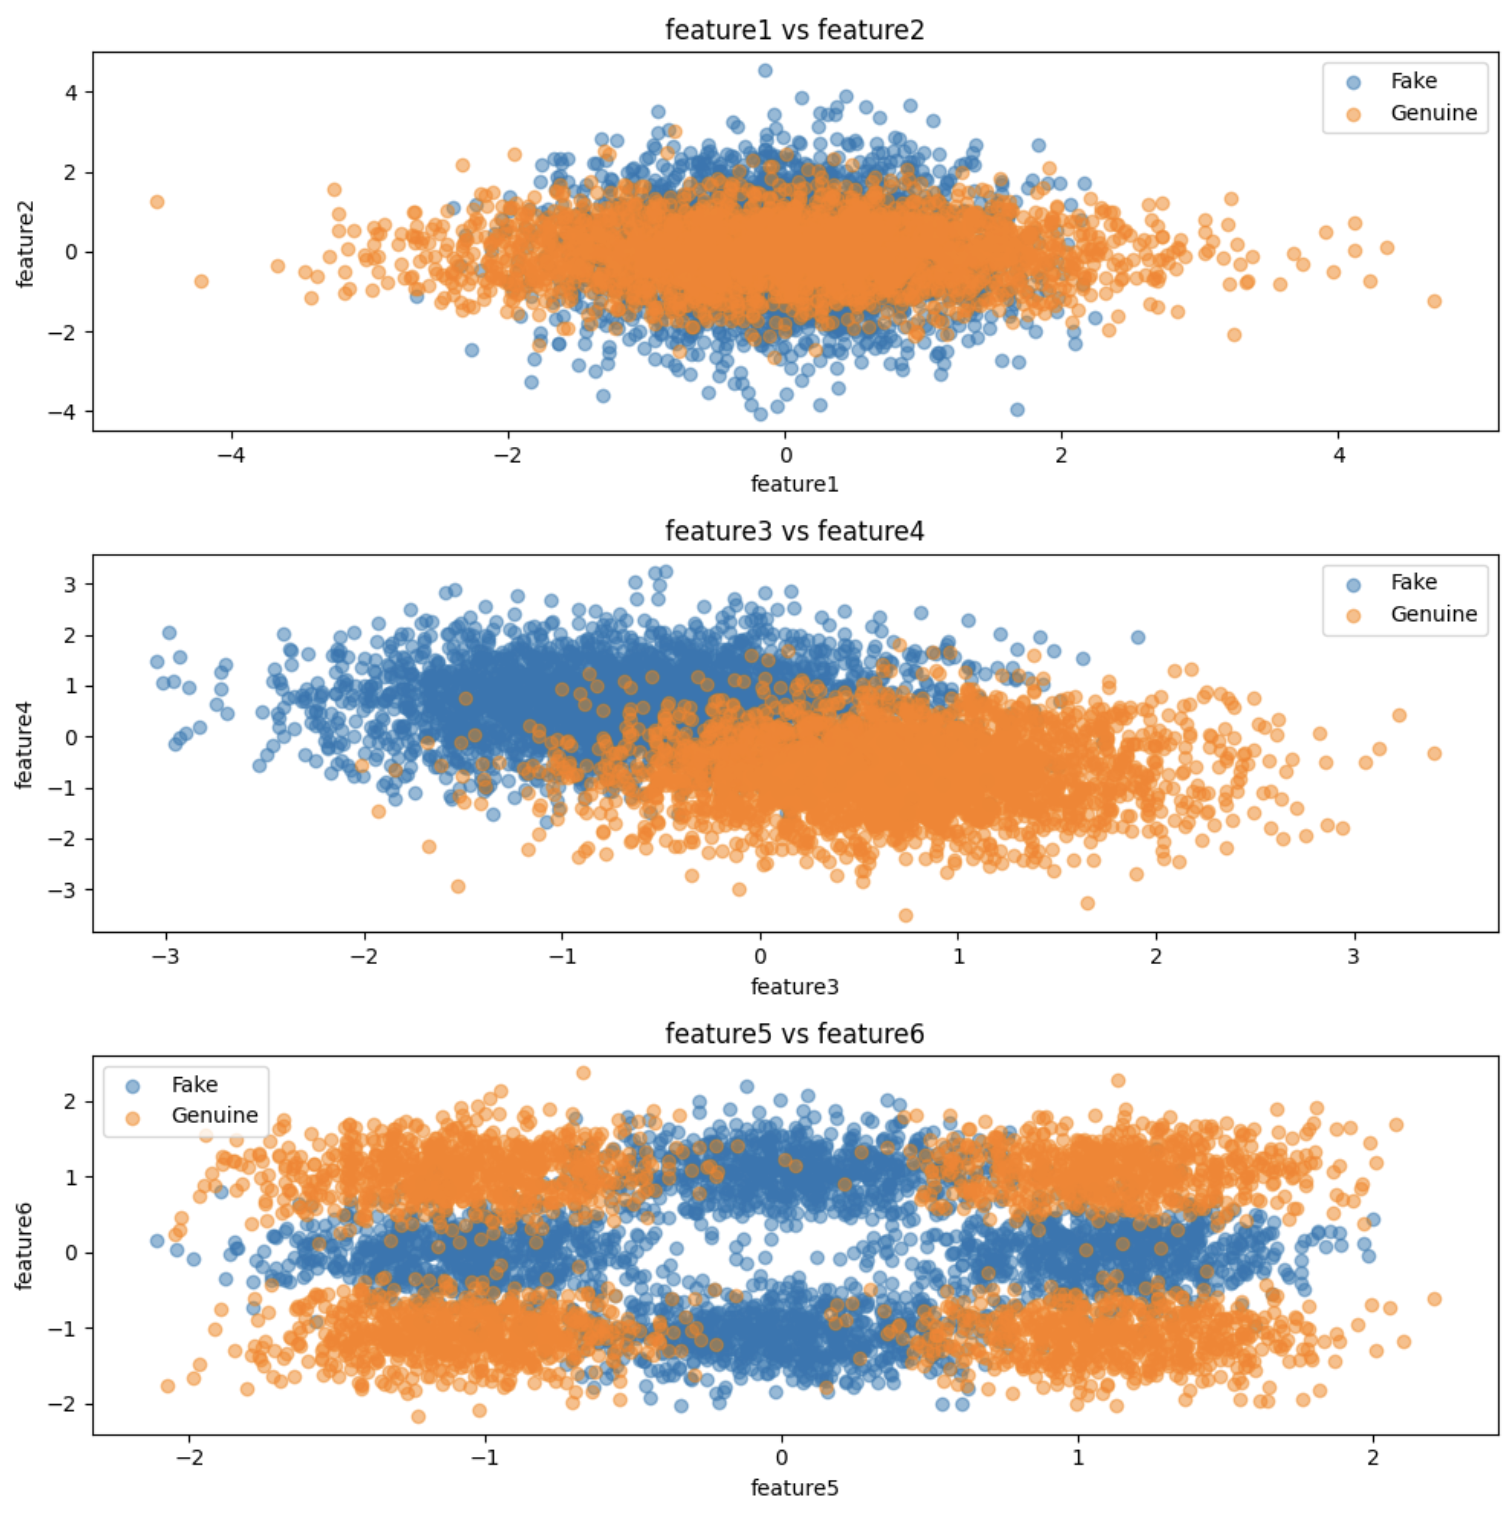
\includegraphics[width=\textwidth]{./img/image2.png}
        \caption{Distribution of feature pairs}
        \label{fig:PairFeatures}
    \end{minipage}
    \hfill % Aggiunge uno spazio orizzontale tra le due minipage se necessario
    \begin{minipage}[b]{0.45\textwidth}
        \centering
        \begin{tabular}{ccc}
            \hline
            Feature & Mean & Variance \\ \hline
            1 & 0.00170711 & 1.00134304 \\
            2 & 0.00503903 & 0.9983527 \\
            3 & -0.00560753 & 1.0024818 \\
            4 & 0.00109537 & 0.99029389\\
            5 & -0.00700025 & 1.00119747 \\
            6 & 0.00910515 & 0.99722374 \\ \hline
        \end{tabular}
        \caption{Mean and variance for each features}
        \label{tab:mean-variance}
    \end{minipage}
\end{figure}
    \\
After making these calculations we can conclude that the data are already centered since all features have mean close to zero.\\
Analyzing the pairwise averages and variances of the features, we can make some observations:  
\begin{itemize}
    \item Feature 1 and Feature 2: These two features have averages very close to zero, indicating that their values are similarly distributed around zero. However, the variance of Feature 2 is slightly lower than that of Feature 1, indicating that the values of Feature 2 are slightly less dispersed than those of Feature 1.  
    \item Feature 3 and Feature 4: Feature 3 has a negative mean, while Feature 4 has a positive mean. This might indicate that the values of Feature 3 tend to be lower than those of Feature 4. Also, the variance of Feature 3 is slightly higher than that of Feature 4, indicating that the values of Feature 3 are more dispersed than those of Feature 4.  
    \item Feature 5 and Feature 6: Feature 5 has a negative mean, while Feature 6 has a positive mean. This might indicate that the values of Feature 5 tend to be lower than those of Feature 6. Also, the variance of Feature 5 is slightly higher than that of Feature 6, indicating that the values of Feature 5 are more dispersed than those of Feature 6. 
\end{itemize}
\subsection{Features correlation}
We can show how correlated the features are by using a heatmap that shows a darker color within the cells for which there is a high correlation between feature i and feature j. The correlation between feature x and feature y is calculated using Pearson's coefficient:
\begin{equation}
    Corr_{i,j} = \frac{Cov(i,j)}{\sqrt{Var(i)}\sqrt{Var(j)}}  
\end{equation}
\begin{figure}[H]
    \centering
    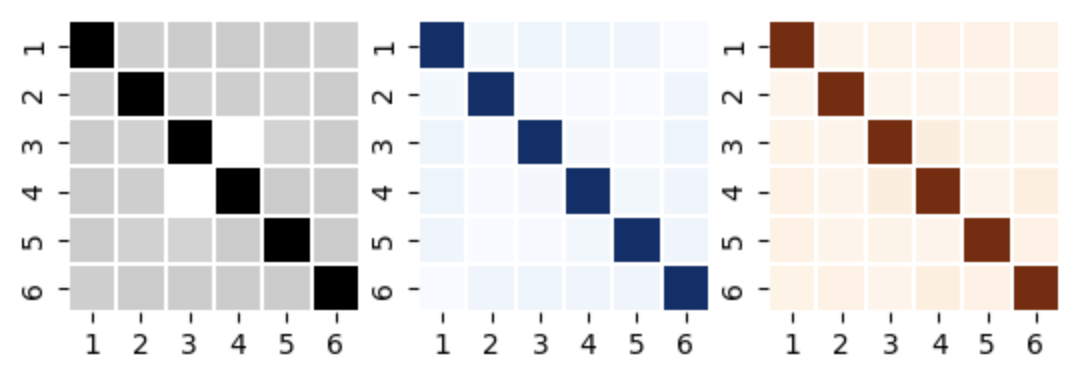
\includegraphics[width=0.8\textwidth]{./img/correlazione.png}
    \caption{Correlation features: gray scale indicates the correlation between whole dataset, blue is for Fake class and orange for Genuine class}
    \label{fig:AllFeatures}
\end{figure} 
Most of the features do not appear to be particularly correlated; in fact, most of the values in the correlation matrix are close to zero.\\
\\
Since the features do not appear to be strongly correlated since precisely the values are close to zero. This suggests to us that each feature carries unique information that could be useful for classification. Therefore, it is most likely that in PCA we will use a value of m as high as possible, possibly equal to the number of features in this way it will be possible to preserve as much of the information in the data as possible.\\
\\
While in the case of Naive Bayes model and Full Covariance Gaussian Model could have similar performance because the features appear to be not strongly correlated. While in the case of the Tied model, which shares the covariance matrix between the classes, it may not have very good performance since the features are not strongly correlated.

\section{Dimensionality reduction}
Dimensionality reduction is useful in this context to compute a mapping from an n-dimensional feature space to an m-dimensional space; it is applied because it can compress information, remove noise and simplify classification.
\subsection{PCA}
PCA is an unsupervised dimensionality reduction technique that, given a centered dataset \\\(X = \{x_1, \ldots, x_k\}\), it aims to find the subspace of \(R^n\) that allows to preserve most of the information, i.e. the directions with the highest variance.
We start by calculating the covariance matrix:
\begin{equation}
\mathbf{C} = \frac{1}{K} \sum_{i} (x_i - \bar{x})(x_i - \bar{x})^T
\end{equation}
After that we can compute the eigen-decomposition of \(
\mathbf{C} = \mathbf{U} \Sigma \mathbf{U}^T,
\)
where \( \mathbf{U} \) is the matrix of eigenvectors and \( \Sigma  \) is the diagonal matrix of eigenvalues. Now we can project the data into the new subspace, it is spanned by the m columns of U corresponding to the m values of the highest eigenvalues.\\
\begin{equation}
\mathbf{y_i} = \mathbf{P^T} (x_i - \bar{x})
\end{equation}
P is the matrix corresponding to the m columns of U associated with the m highest eigenvalues of C.
At this point to choose which is the best value of m we need to check how much total variance in the data we are able to retain using different values of m.
To do this evaluation, it was decided to represent on a graph the variance of the data as m increases, i.e., we exploited that each eigenvalue corresponds to the variance along the corresponding axis, and the eigenvalues are the elements of the diagonal of the matrix \(\Sigma\) . The percentage will be calculated as the ratio of the sum of the first m eigenvalues to the sum of all eigenvalues.
\begin{figure}[H]
    \centering
    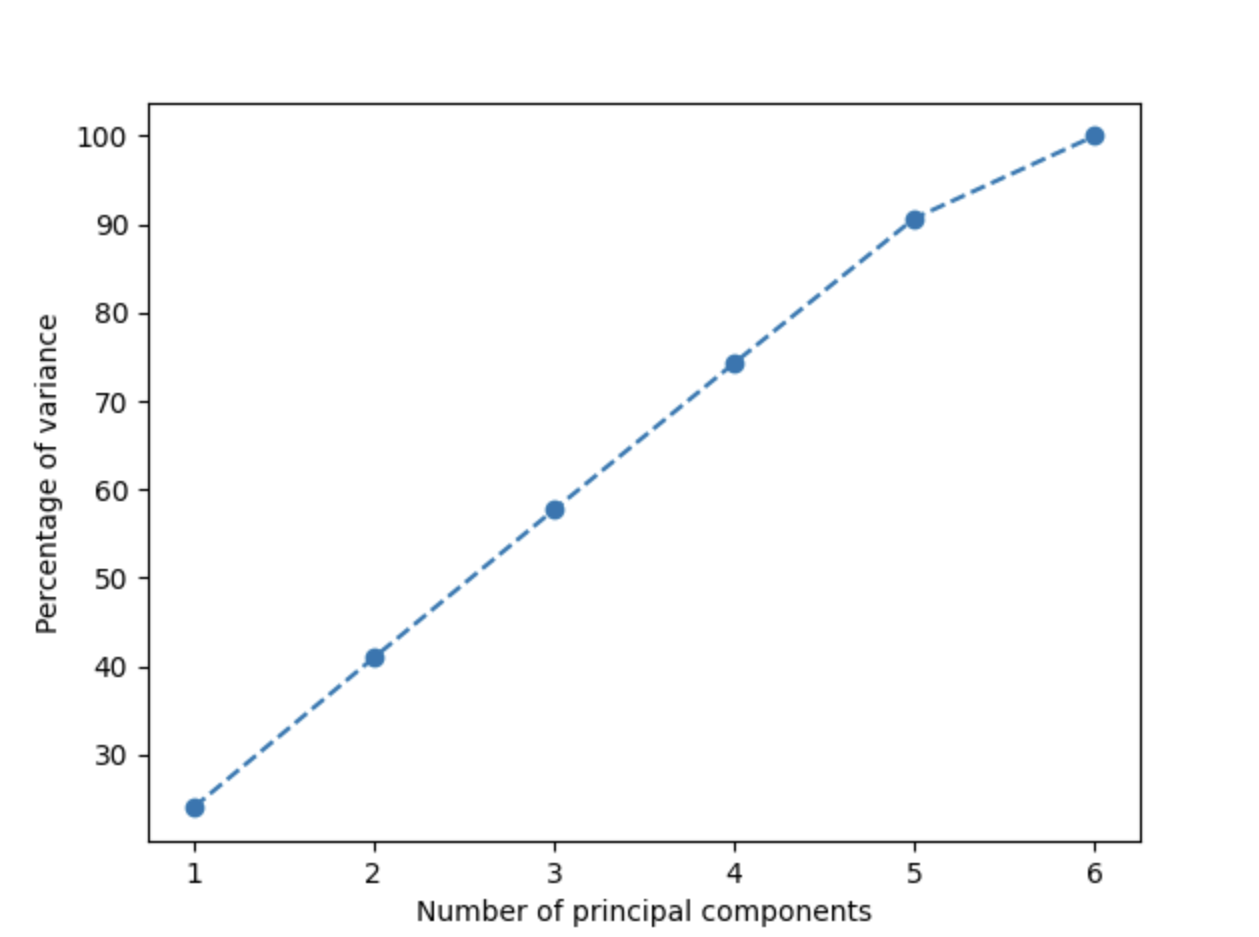
\includegraphics[width=0.5\textwidth]{./img/variance.png}
    \caption{Variance of data for each m values}
    \label{fig:variance}
\end{figure} 

It is clear from Figure~\ref{fig:variance} that values of \( m<5\) rapidly decrease the amount of variance retained in the data. Removing a feature is probably the best choice, since this way the percentage of variance remains fairly high.
\begin{figure}[H]
    \centering
    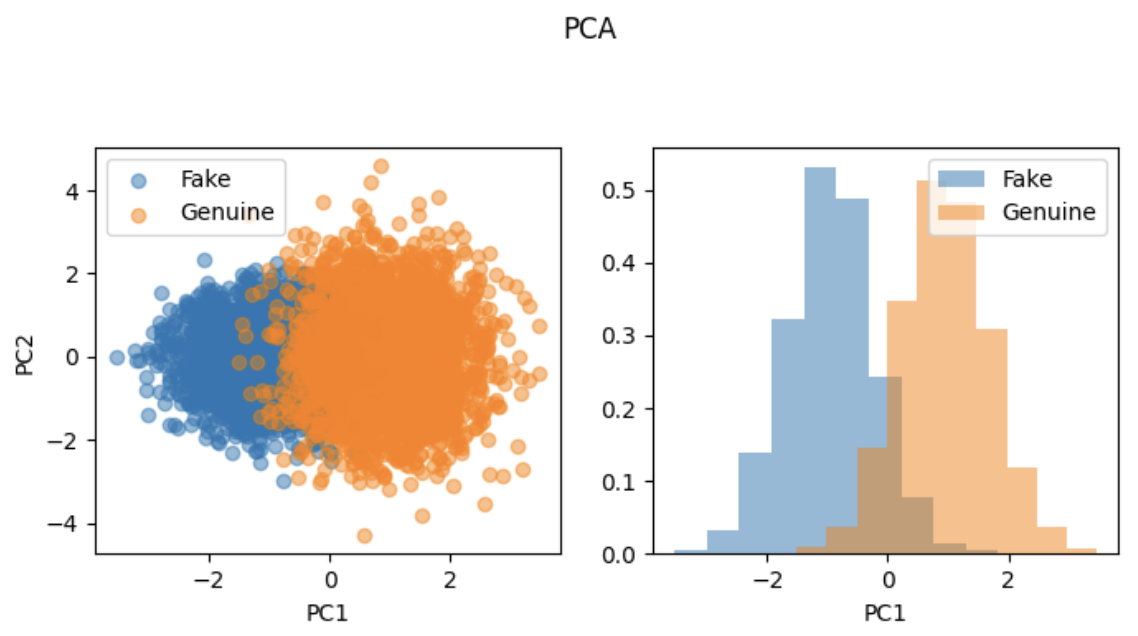
\includegraphics[width=0.7\textwidth]{./img/PCA.png}
    \caption{PCA for the two first components}
    \label{fig:PCA}
\end{figure} 

After the analysis done to choose which m is best to use, we can represent the first two principal components found by calculating the PCA with m=6, visualizing these components can help to understand which features contribute most to the variance in the data.
It can actually be observed that there is better separation between classes by applying PCA and choosing an m that has good variance of the data.
\subsection{LDA}
LDA is a supervised dimensionality reduction technique that aims to find the subspace that maximizes the separation between classes. \\
To compute the transformation matrix \( W \) we need to compute between-class and within-class covariance matrices.
\begin{equation}
\mathbf{S}_b =\frac{1}{N}\sum_{c=1}^{K} n_c (\mu_c - \mu)(\mu_c - \mu)^T
\end{equation}
\begin{equation}
    \mathbf{S}_w = \frac{1}{N}\sum_{c=1}^{K} \sum_{i=1}^{n_c} (x_{c,i} - \mu_i)(x_{c,i} - \mu_i)^T
    \end{equation}
where \( \mu_c \) is the mean of the c-th class, \( \mu \) is the mean of all the data, and \( n_c \) is the number of samples in the c-th class.\\
The LDA directions can be computed solving the generalized eigenvalue problem \(S_b w=\lambda S_w w\), usually to solve the generalized eigenvalue problem we transform the \(S_w\) matrix into an identity matrix and then solve the eigenvalue problem for the other \(S_b \) matrix. This process allows us to find the discriminant vectors \(w\) that maximize the separation between the classes.\\
In LDA, the maximum number of discriminant directions or dimensions that can be obtained is always equal to C-1 where C is the number of classes. This is because the goal of the LDA is to find the directions that maximize the separation between the classes. 
In our case having only two classes the LDA can find at most one direction that maximizes the separation between these two classes.
\begin{figure}[H]
    \centering
    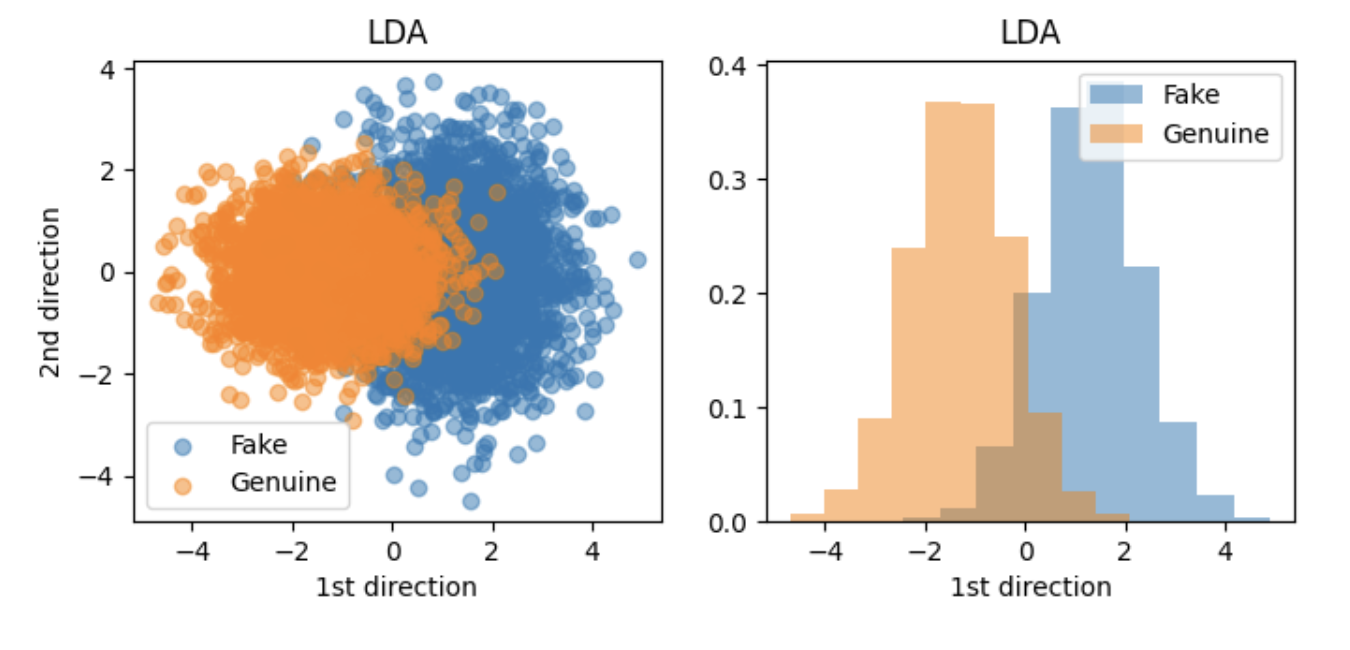
\includegraphics[width=0.7\textwidth]{./img/LDA.png}
    \caption{LDA for first direction}
    \label{fig:LDA}
\end{figure} 
Looking at the results of LDA, in Figure~\ref{fig:LDA}, we can see that it cannot find an optimal direction that gives us a better separation of classes than the results shown previously.
\subsection{Classification}
Subsequent to applying dimensionality reduction techniques we used LDA to perform classification, in fact after finding the hyperplane on the training data and projecting the validation data into the new space we used different thresholds to perform classification.
After applying dimensionality reduction techniques, we used LDA to perform classification; in fact, after finding the hyperplane on the training data and projecting the validation data into the new space these new data values can be used as scores by comparing them with different thresholds to perform classification, if the value exceeds the threshold it is associated with the label 1 while if it is lower 0.
Two different methods were used to calculate the threshold value:
\begin{itemize}

\item \textbf{First Threshold}: The first method calculates the average of the LDA values for the two classes and uses the average of these two averages as the threshold. This method is simpler, but does not take into account the distribution of the data or the classification error rate. In fact, it may not provide an optimal threshold if the data are not well balanced or if the distributions of the two classes overlap significantly.
\item \textbf{Second Threshold}: The second method uses a more sophisticated approach to determine the threshold. Instead of simply calculating the mean, a range of possible threshold values are examined and the one that minimizes the classification error rate is chosen. This method is more computationally heavy, but can lead to a more accurate threshold and a lower classification error rate.  
\end{itemize}
\begin{table}[H]
    \centering
    \begin{tabular}{lcc}
    \hline
    \textbf{Methods} & \textbf{Number of errors} & \textbf{Error rate (\%)} \\
    \hline
    LDA - First threshold & 275 & 13.75 \\
    LDA - Second threshold & 184 & 9.2 \\
    \hline
    PCA(m=6)+LDA - First threshold & 186 & 9.3 \\
    PCA(m=5)+LDA - First threshold & 186 & 9.3 \\
    PCA(m=6)+LDA - Second threshold & 184 & 9.2 \\
    PCA(m=5)+LDA - Second threshold & 185 & 9.25 \\
    \hline
    \end{tabular}
    \caption{LDA and PCA+LDA results with different threshold}
    \label{tab:resultsPCALDA}
\end{table}
As can be seen from the Table~\ref{tab:resultsPCALDA} there is not much real improvement by applying PCA as pre-processing before LDA and that the classification error turns out to be quite high so good classification is not performed using LDA or the combination of LDA with PCA.


\section{Multivariate Gaussian Density}
The multivariate Gaussian distribution is a generalization of the multidimensional Gaussian normal distribution. It is used to describe the probability of a vector of continuous random variables that can be correlated with each other.\\
The multivariate Gaussian distribution in d dimensions is characterized by a vector of averages \(\mu\)  and a covariance matrix \(\Sigma\). The probability density function of the multivariate Gaussian distribution is given by:
\begin{equation}
    \mathcal{N}(x|\mu,\Sigma ) = \frac{1}{(2\pi)^{M/2}|\Sigma|^{1/2}} \exp\left(-\frac{1}{2}(x-\mu)^T\Sigma^{-1}(x-\mu)\right)
\end{equation}
Very often to prevent numerical problems due to exponentiation of large numbers, it is usually recommended to work on the logarithm of the density:
\begin{equation}
    \log \mathcal{N}(x|\mu,\Sigma ) = - \frac{M}{2} \log(2\pi) -\frac{1}{2} \log |\Sigma| - \frac{1}{2}(x-\mu)^T\Sigma^{-1}(x-\mu) 
\end{equation}
\begin{figure}[H]
    \centering
    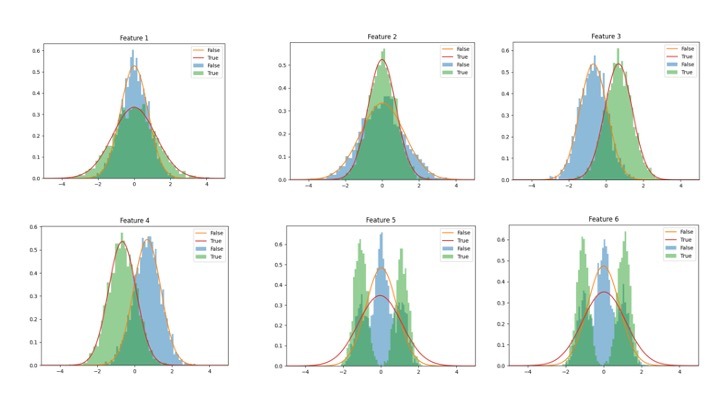
\includegraphics[width=0.8\textwidth]{./img/GaussianDensity.jpeg}
    \caption{Gaussian density}
    \label{fig:gaussianD}
\end{figure} 
The curve we can observe on the graph in Figure~\ref{fig:gaussianD} represents the Gaussian probability density calculated from the data. If the data actually follow a Gaussian distribution, then the curve should fit the histogram of the data well. When this happens we can say that the Gaussian model is a good fit for the data while if the Gaussian curve does not fit the histogram well, then the Gaussian model may not be the most appropriate model for that data.\\
We can observe that feature 1, feature 2, feature 3 and feature 4 fit the model well and follow a Gaussian distribution.
\section{Model evaluation for classification}
To understand which model is the most promising and gives us the best results, we divided the dataset as mentioned above into a part for training and a part for validation. This way we can test our model on data other than the training data.\\
We considered different types of applications i.e. various values of (\( \tilde{\pi},C_{fn},C_{fp})\). The target application chosen to be balanced will be:
\begin{equation}
    (\tilde{\pi},C_fp,C_fn) = (0.1,1,1)
\end{equation}
The objective of the following analysis is to choose the model with the best performance. Performance will be measured in terms of normalized minimum detection costs. This technique would allow us to discriminate the best performing model for our target application by providing an assessment of how well the model can detect the class to which it belongs. 
\\
It is defined as follows:
\begin{equation}
    DCF_u= \sum_{k=0}^{K-1} \frac{\pi_k}{N_k} \sum_{i|c_i=k}C(c_i^*|k)=\pi_TC_{fn} P_{fn}+(1-\pi_T)C_{fp}P_{fp} 
\end{equation}
\label{eq:DCF}
where \(P_{fn}=\frac{FN}{FN+FP}\) and \(P_{fp}=\frac{FP}{FP+TP}\).\\
\\
From the Equation~\ref{eq:DCF}  it is possible to find \textbf{minDCF} and \textbf{actDCF}, and different thresholds are used to calculate these. In fact in the case of minDCF one uses as a threshold the one that minimizes DCF and there are several methods to be able to find it. Whereas for actDCF you use as a threshold:
\begin{equation}
    t'=-\log{\frac{\tilde{\pi}}{1-\tilde{\pi}}}
\end{equation}

\section{Classification model analysis}
To perform the classification obviously we had to divide the training dataset into a part for training and a part for validation.

\subsection{Gaussian Models}
The first class of models we will analyze is that of Gaussian generative models. A simple model is to assume that our data, given a class, can be described by a Gaussian distribution:
\begin{equation}
    f_{x|C}(x|c) = \mathcal{N}(x|\mu_c,\Sigma_c)
\end{equation}
Since this is a binary classification task, we will assign a probability score to each sample in terms of the log-posterior class likelihood ratio:
\begin{equation}
    llr(x_t) = \log \;r(x_t) = \log \frac{P(C=h_1|x_t)}{P(C=h_0|x_t)}
\end{equation}
This expression can be expanded writing:
\begin{equation}
    llr(x_t) = \log \frac{f_{X|C}(x_t|C=h_1)}{f_{X|C}(x_t|C=h_1)} + \frac{\pi }{1-\pi }
\end{equation}
where \( f_{X|C}(x_t|c)=\mathcal{N}(x|\mu_c,\Sigma_c)\)\\\\
It is necessary to find the parameters \(\theta \), \(\mu_c\) and \(\Sigma_c \); this can be done by maximizing the log-likelihood.\\ Parameter estimation is part of the training phase and is therefore performed on the training part of the dataset.
While the estimation phase is to calculate the likelihood ratio for each sample and compare it to a threshold, which will be set at 0(th=0) in this step. After doing this, the error rate can be calculated to evaluate the classification. 
This analysis has been done on different Gaussian models, the difference between these models is the way the parameters \((\mu_c ,\Sigma_c )\) are calculated, more specifically \(\Sigma_c\).
\subsubsection{MVG Gaussian Classifier}
The first model we will analyze is the multivariate Gaussian classifier; in this model the covariance matrix is assumed to be different for each class. The parameters \(\mu_c\) and \(\Sigma_c\) are estimated by maximizing the log-likelihood of the training data. Thus they can be obtained as:
\begin{equation}
    \mu_c^* = \frac{1}{N_c} \sum_{i|c_i=C} x_{i} \;\;\;\;\; \sigma_c^* = \frac{1}{N_c} \sum_{i|c_i=C} (x_{i} - \mu_c)(x_{i} - \mu_c)^T
\end{equation}
\subsubsection{Naive Bayes Classifier}
The Naive Bayes hypothesis simplifies the MVG full covariance model. In fact, if we know that the different components of our characteristics are approximately independent, we can simplify the estimation by assuming that the distribution of x|C can be factorized on its components.\\
The parameters then become:
\begin{equation}
    \mu_{c,[j]}^* = \frac{1}{N_c} \sum_{i|c_i=C} x_{i,[j]} \;\;\;\;\; \sigma_{c,[j]}^* = \frac{1}{N_c} \sum_{i|c_i=C} (x_{i,[j]} - \mu_{c,[j]})^2
\end{equation}
The Naïve Bayes classifier corresponds to the MVG full covariance classifier with a diagonal covariance matrix.
\subsubsection{Tied Bayes Classifier}
Another common Gaussian Model is Tied Model, it assumes that the covariance matrix is the same for all classes, but each class still has its own mean.
It assumes that:
\begin{equation}
    f_{X|C}(x|c) = \mathcal{N}(x|\mu_c,\Sigma)
\end{equation}
While the parameters are estimated as:
\begin{equation}
    \mu_c^* = \frac{1}{N_c} \sum_{i|c_i=C} x_{i} \;\;\;\;\; \Sigma^* = \frac{1}{N} \sum_{c} \sum_{i|c_i=C} (x_{i} - \mu_c)(x_{i} - \mu_c)^T
\end{equation}
where \(N= \sum_{c=1}^{k}Nc\), that is the number of all samples.\\
This model is strongly related to LDA, if considering the binary log-likelihood ratio of the tied model we obtain a linear decision function:
\begin{equation}
    llr(x_t) = log \frac{f_{X|C}(x|h_1)}{f_{X|C}(x|h_0)}= x^Tb+c
\end{equation}
where b and c are functions of class means and covariance matrix. On the other hand, projecting
over the LDA subspace is, up to a scaling factor k, given by:
\begin{equation}
   w^tx=k x^T \Lambda (\mu_1-\mu_0)
\end{equation}

where \( \Lambda(\mu_1-\mu_0)=b\). The LDA assumption that all the classes have the same within class covariance matrix is related to the assumption done for the tied model.
\subsubsection{Gaussian Models Comparison}
At this point placing the \( P(C = 1) = P(C = 0) = 1/2\), classification was performed as can be seen in Table~\ref{tab:error_ratesMVG} using Gaussian models. 
\begin{table}[H]
    \centering
    \begin{tabularx}{0.6\textwidth}{>{\centering\arraybackslash}l>{\centering\arraybackslash}X>{\centering\arraybackslash}X} 
    \hline
    \textbf{Features} & \textbf{Model} & \textbf{Error Rate (\%)} \\
    \hline
    \multicolumn{3}{c}{no PCA} \\
    \hline
    1,2,3,4,5,6 & Full Cov & 7.00 \\
    1,2,3,4,5,6 & Naïve Bayes &  7.20 \\
    1,2,3,4,5,6 & Tied Cov &  9.30 \\
    \hline
    1,2,3,4 & Full Cov & 7.95 \\
    1,2,3,4 & Naïve Bayes &  7.65 \\
    1,2,3,4 & Tied Cov &  9.50 \\
    \hline
    1,2 & Full Cov &  36.50 \\
    1,2 & Naïve Bayes &  36.30 \\
    1,2 & Tied &  49.45 \\
    \hline
    3,4 & Full Cov &  9.45 \\
    3,4 & Naïve Bayes &  9.45 \\
    3,4 & Tied Cov &  9.40 \\
    \hline
    \multicolumn{3}{c}{PCA m= 5} \\
    \hline
    1,2,3,4,5,6 & Full Cov & 7.10 \\
    1,2,3,4,5,6 & Naïve Bayes & 8.75 \\
    1,2,3,4,5,6 & Tied Cov &  9.30 \\
    \hline
    \multicolumn{3}{c}{PCA m= 6} \\
    \hline
    1,2,3,4,5,6 & Full Cov &  7.00 \\
    1,2,3,4,5,6 & Naïve Bayes &  8.90 \\
    1,2,3,4,5,6 & Tied Cov &  9.30 \\
    \hline
    \end{tabularx}
    \caption{Error Rates for Different Models and Features}
    \label{tab:error_ratesMVG}
    \end{table}
Comparing the results with Table~\ref{tab:resultsPCALDA} , where LDA had been used for classification we can observe that for certain configurations there was an improvement. This could be due to the fact that this method is able to classify better and thus recognize the point to which class it belongs.
Analyzing the data provided in Table~\ref{tab:error_ratesMVG} we can make some considerations about the features used for classification:
\begin{itemize}
    \item \textbf{Features (1,2,3,4,5,6)}: the classification error is relatively low for all models, this may suggest that all features provide useful information.
    \item \textbf{Features (1,2,3,4)}: the classification error increases slightly, so it can be said that features 5 and 6 probably contain useful classification information.
    \item \textbf{Features (1,2),(3,4)}: the classification error increases significantly in the case of features(1,2) because they do not contain particularly important information for classification. While for (3,4),the error remains similar to the others , this might indicate that these two features are particularly informative for classification.  
\end{itemize}

Now we apply to estimate performance the metrics described in the previous section, we began by testing several applications to understand how changing parameters were reflected in performance. 
The prior value represents the a priori probability of the positive class, so if it is higher the value is expected to be more common, while a higher value of \(C_{fn}\) indicates that the cost of misclassifying a positive point as negative is higher, and vice versa for \(C_{fp}\).  
\begin{table}[H]
    \centering
    \begin{tabular}{>{\centering\arraybackslash}m{2cm} >{\centering\arraybackslash}m{2cm} >{\centering\arraybackslash}m{3cm}>{\centering\arraybackslash}m{2cm}}
    \hline
    \textbf{Model}  & \textbf{Full Cov} & \textbf{Naïve Bayes} & \textbf{Tied Cov} \\ \hline
    \rowcolor{yellow}
    \multicolumn{4}{c}{\textbf{Application(\(\pi_T,C_{fn},C_{fp}\)) : (0.50, 1, 1)}} \\   \hline
    \textbf{actDCF} & 0.141913 & 0.174987 & 0.186044 \\
    \textbf{minDCF} & 0.133144 & 0.173691 & 0.181163 \\ \hline
    \rowcolor{yellow}
     \multicolumn{4}{c}{\textbf{Application(\(\pi_T,C_{fn},C_{fp}\)) : (0.90, 1, 1)}} \\   \hline
    \textbf{actDCF} & 0.398041 & 0.466014 & 0.462558 \\
    \textbf{minDFC} & 0.351238 & 0.434044 & 0.445132 \\ \hline
    \rowcolor{yellow}
    \multicolumn{4}{c}{\textbf{Application(\(\pi_T,C_{fn},C_{fp}\)) : (0.10, 1, 1)}} \\   \hline
    \textbf{actDCF} & 0.304147 & 0.393017 & 0.405066 \\
    \textbf{minDFC} & 0.273825 & 0.354471 & 0.364823 \\ \hline
    \multicolumn{4}{c}{\textbf{Application(\(\pi_T,C_{fn},C_{fp}\)) : (0.50, 1, 9)}} \\   \hline
    \textbf{actDCF} & 0.304147 & 0.393017 & 0.405066 \\
    \textbf{minDFC} & 0.273825 & 0.354471 & 0.364823 \\ \hline

    \multicolumn{4}{c}{\textbf{Application(\(\pi_T,C_{fn},C_{fp}\)) : (0.50, 9, 1)}} \\   \hline
    \textbf{actDCF} & 0.398041 & 0.466014 & 0.462558 \\
    \textbf{minDFC} & 0.351238 & 0.434044 & 0.445132 \\ \hline
    \end{tabular}
    \caption{minDCF and actDCF for Different Models and configurations}
    \label{tab:model_comparison}
    \end{table}
    So it can be seen from the Table~\ref{tab:model_comparison} that:
    \begin{itemize}
        \item When the value of Prior increases (from 0.50 to 0.90), a worsening of the models can be seen. This is due to the fact that the model is penalizing false negatives more heavily. This also happens when Prior decreases and therefore you are penalizing false positives more heavily.
        \item When Cfp increases to 9.00 , the actDCF and minDCF of all models do not change compared to the case when Cfp is 1.00. This suggests that increasing the cost of false positives does not have a significant impact on model performance.  While
        if Cfn increases to 9.00 , the DCFAct and minDCF of all models increase compared to the case where Cfn is 1.00, from this we can derive that the increase in the cost of false negatives worsens the performance of the models.
    \end{itemize}
We now focus on the three applications that have different effective priors (0.1, 0.5, 0.9) and with costs of errors equal to 1.00.\\
    
    
\subsection{Logistic Regression Classifier}
\subsubsection{Quadratic Logistic Regression(QLR)}
\subsection{SVM Classifier}
\subsubsection{Linear SVM}
\subsubsection{Kernel SVM}
\subsection{GMM Classifier}
\section{Score Calibration}
\subsection{Calibration Analysis on Selected Models}
\subsection{Calibrating Scores for Selected Models}
\section{Experimental Results}
\subsection{Calibration on evaluation score}
\subsection{Considerations}
\section{Conclusions}


\newpage



% ------------------------------------------------------------------------------

\end{document}
